%%% Main Figures

\subsection*{Figures}

\begin{figure}[H]
    %\includegraphics[width=\linewidth]{fig/MainFigures/Fig1.pdf}
    \caption{
      \textbf{IMPG: implicit pangenome graph concept and distributed construction.}
      \textbf{A.} Conceptual overview: pairwise alignments implicitly define a graph structure through transitive match relationships. IMPG indexes alignments using cache-oblivious interval trees and discovers sequences related through multi-hop alignment chains without materializing the graph.
      \textbf{B.} Partition-lace pipeline for distributed pangenome construction. Unlike chromosome-based or whole-sequence community approaches, alignment-based partitioning operates at interval granularity: individual contigs can be split across partitions at alignment boundaries, correctly handling translocations and rearrangements. Partitions are independently processed through graph construction or variant calling tools, then merged into unified GFA or VCF files.
    }
    \label{fig:concept}
\end{figure}

\begin{figure}[H]
    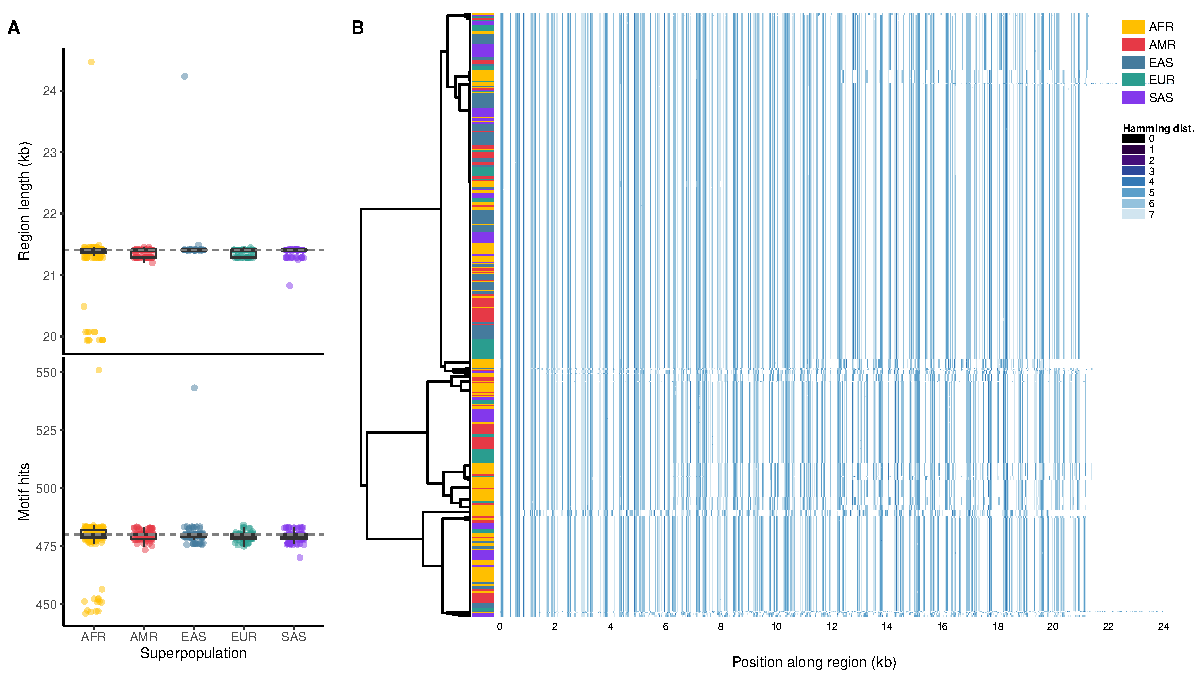
\includegraphics[width=\linewidth]{fig/MainFigures/Fig2.pdf}
    \caption{
      \textbf{EBV-associated tandem repeat polymorphism at 11q23 across 466 human haplotypes.}
      \textbf{A.} Distribution of repeat region lengths (top) and EBNA1-like motif hit counts (bottom) at the chr11q23 tandem repeat cluster across all HPRCv2 haplotypes, colored by superpopulation.
      \textbf{B.} EBNA1-like motif hit positions across all haplotypes, displayed as a binary heatmap (20\,bp bins) with rows ordered by hierarchical clustering (Ward's method on binary distance). Superpopulation annotation is shown as a color bar; the dendrogram reveals structural clusters that do not segregate strictly by ancestry.
    }
    \label{fig:ebv}
\end{figure}
